\documentclass[12pt,a4paper]{article}

\usepackage[in, plain]{fullpage}
\usepackage{array}
%\usepackage{../../../pas-math}
\usepackage{../../../moncours2}


%\author{Olivier FINOT}
\date{}
\title{\textcircled{{\normalsize{7}}} Angles et parallélisme}

\graphicspath{{./img/}}



\begin{document}
\maketitle




%\chap[num=9, color=red]{Angles et parallélisme}{}

\begin{myobj}
	\begin{itemize}
		
		\item Construire le symétrique d’un point ou d'une figure par rapport à une droite à la main où à l’aide d’un logiciel;
		\item Construire le symétrique d’un point ou d'une figure par rapport à un point, à la main où à l’aide d’un logiciel;
		\item Utiliser les propriétés de la symétrie axiale ou centrale;
		\item Identifier des symétries dans des figures.		
	\end{itemize}
\end{myobj}

\begin{mycomp}
	\begin{itemize}
		\item \kw{Chercher (Ch2)} :  s’engager    dans    une    démarche    scientifique, observer, questionner, manipuler, expérimenter (sur une feuille de papier, avec des objets, à l’aide de logiciels), émettre des hypothèses, chercher des exemples ou des contre-exemples, simplifier ou particulariser une situation, émettre une conjecture ;
		\item \kw{Raisonner (Ra3)} :  démontrer : utiliser un raisonnement logique et des règles établies (propriétés, théorèmes, formules) pour parvenir à une conclusion ;
		\item \kw{Communiquer (Co2)} :  expliquer à l’oral ou à l’écrit (sa démarche, son raisonnement, un calcul, un protocole   de   construction   géométrique, un algorithme), comprendre les explications d’un autre et argumenter dans l’échange ; 
		
	\end{itemize}
\end{mycomp}





\section{Angles opposés par le sommet}


\begin{mydef}
	Deux angles ayant le même sommet et sont dans le prolongement l'un de l'autre, alors ils sont \kw{opposés par le sommet}
\end{mydef}

\begin{myprop}
	Deux angles opposés par le sommet ont la \kw{même mesure}.
\end{myprop}


\begin{myex}
	
	\begin{multicols}{2}
		les droites $(AB)$ et $(CD)$ sécantes en $O$ forment deux paires d'angles opposés par le sommet.
		
		On a :
		\begin{itemize}
			\item $\widehat{AOC} = \widehat{BOD}$
			\item $\widehat{AOD} = \widehat{BOC}$
		\end{itemize}	
	
		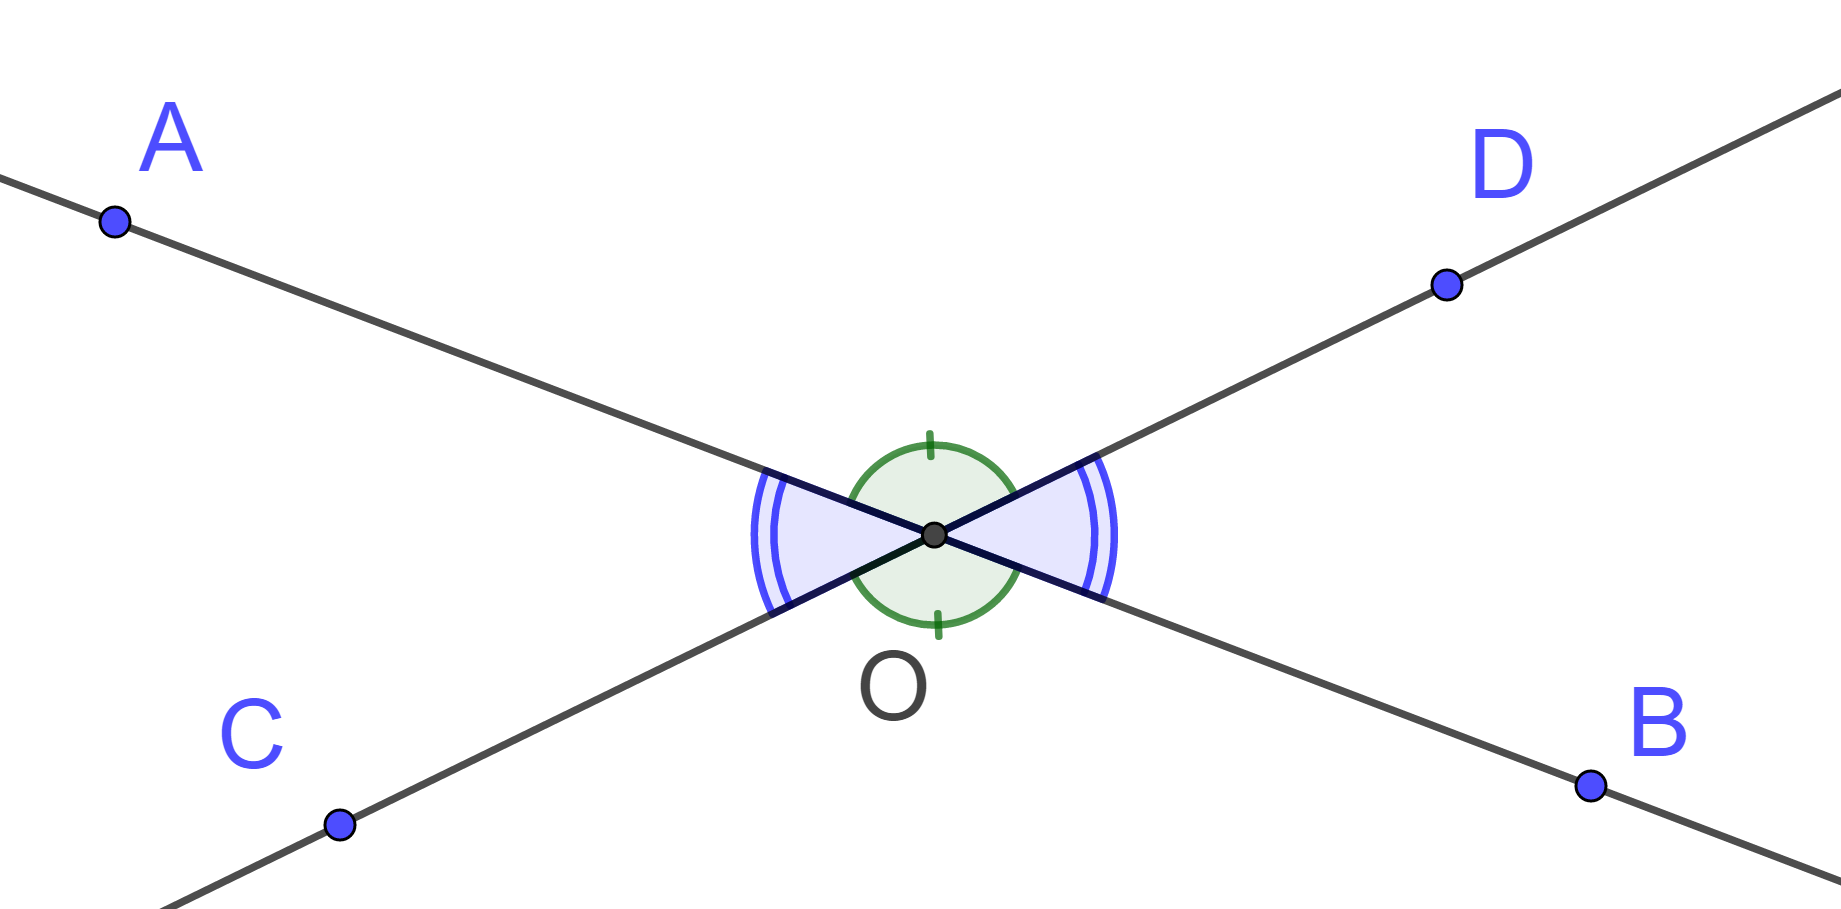
\includegraphics[scale=0.15]{opposes}
	\end{multicols}
	
\end{myex}
\section{Angles alternes-internes}


\begin{mydef}
	
	
		Soit deux droites $(d_1)$ et $(d_2)$, une troisième droite $(s)$, les coupe en $A$ et $B$.
		Dans angles formés par ces 3 droites sont alternes-internes si et seulement si :
		
		\begin{multicols}{2}
		\begin{itemize}
			\item ils ont pour sommet $A$ et $B$;
			\item ils sont de part et d'autre de la droite $(s)$;
			\item ils sont entre les droites $(d_1)$ et $(d_2)$.
		\end{itemize}
	
	
		\begin{center}
			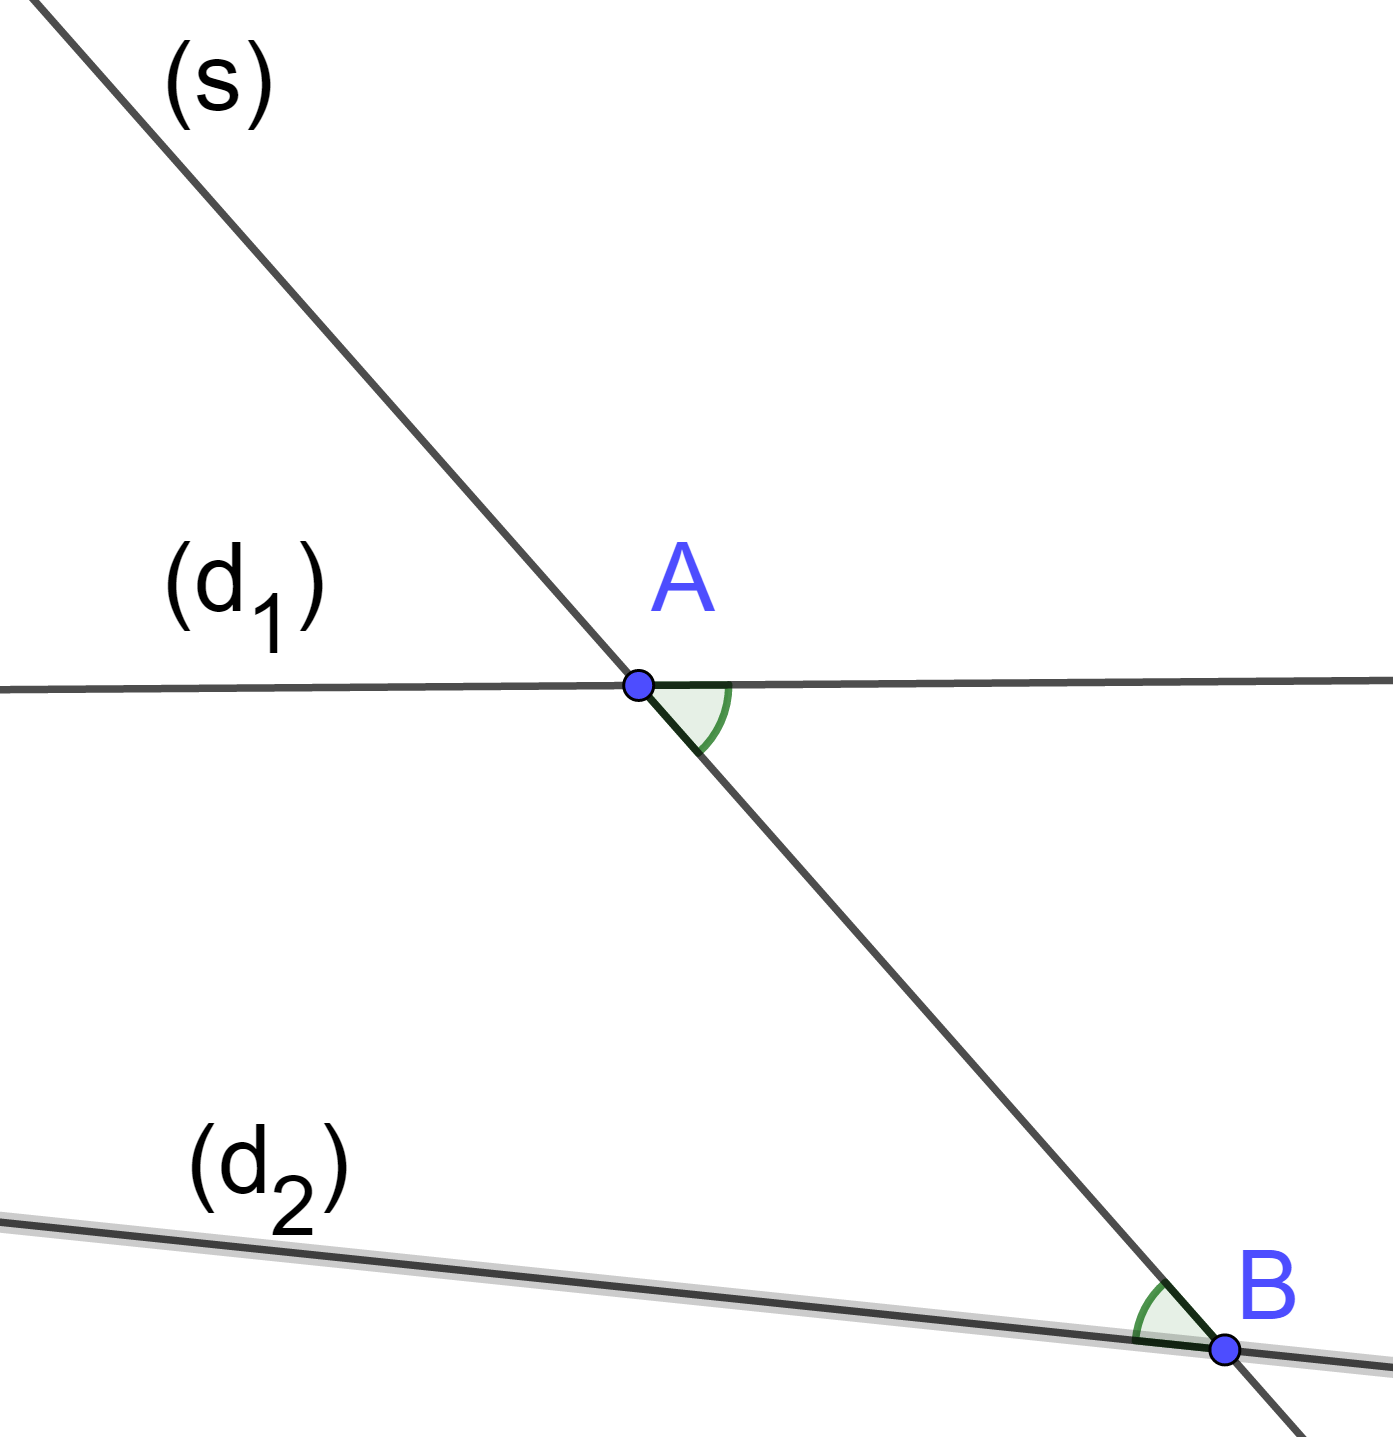
\includegraphics[scale=0.14]{alt_int}
		\end{center}
	\end{multicols}

\end{mydef}


\begin{myprop}
	Si deux droites coupées par une sécante sont \kw{parallèles}, alors les angles alternes-internes ont \kw{la même mesure}.
\end{myprop}

\begin{myex}
	
	
	\begin{multicols}{2}
		Les droites $(AE)$ et $(BC)$ sont parallèles et les angles $\widehat{EAB}$ et $\widehat{ABC}$ sont alternes-internes. \\
		
		Donc les angles $\widehat{EAB}$ et $\widehat{ABC}$ ont la même mesure.
		
		\begin{center}
			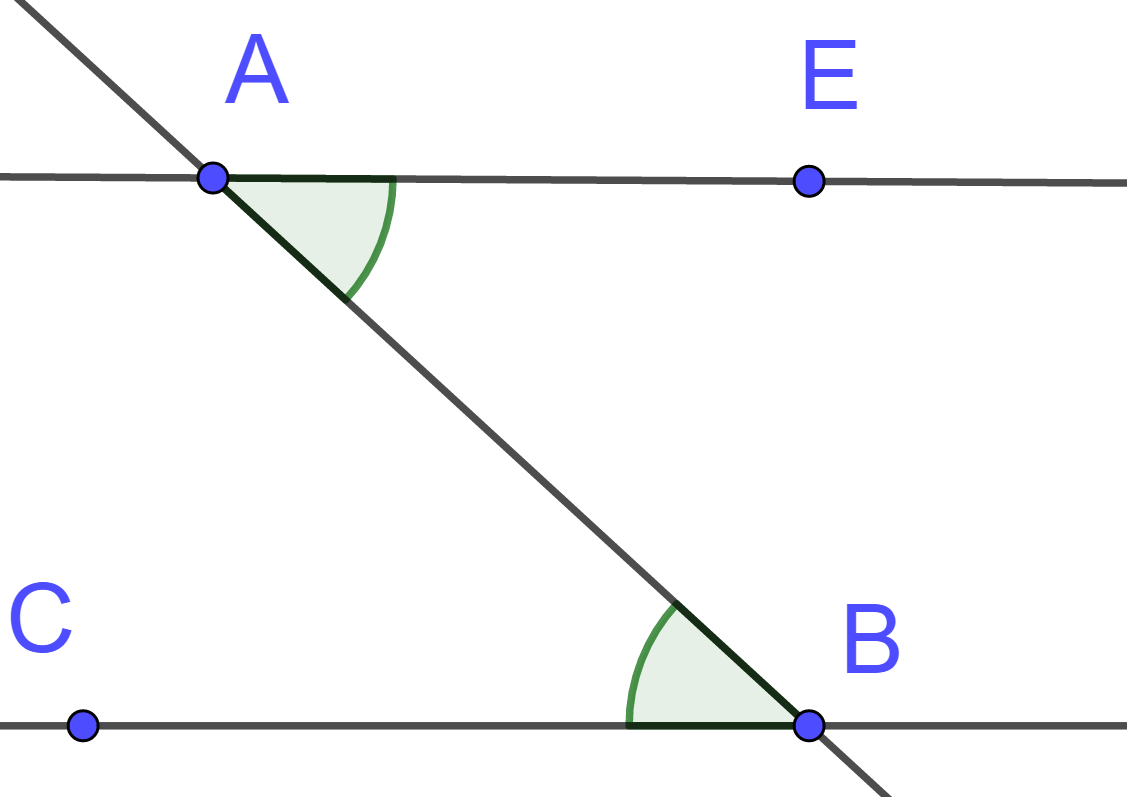
\includegraphics[scale=0.15]{alt_int2}
		\end{center}
	\end{multicols}
\end{myex}


\begin{myprop}
	Si deux angles alternes-internes ont \kw{la même mesure}, alors les droites coupées par la sécante sont \kw{parallèles}.
\end{myprop}

\begin{myex}
	\begin{multicols}{2}
		
		Les angles $\widehat{AEC}$ et $\widehat{BCE}$ sont alternes-internes et de même mesure. \\
		
		Donc les droites $(AE)$ et $(BC)$ sont parallèles.
		
		\begin{center}
			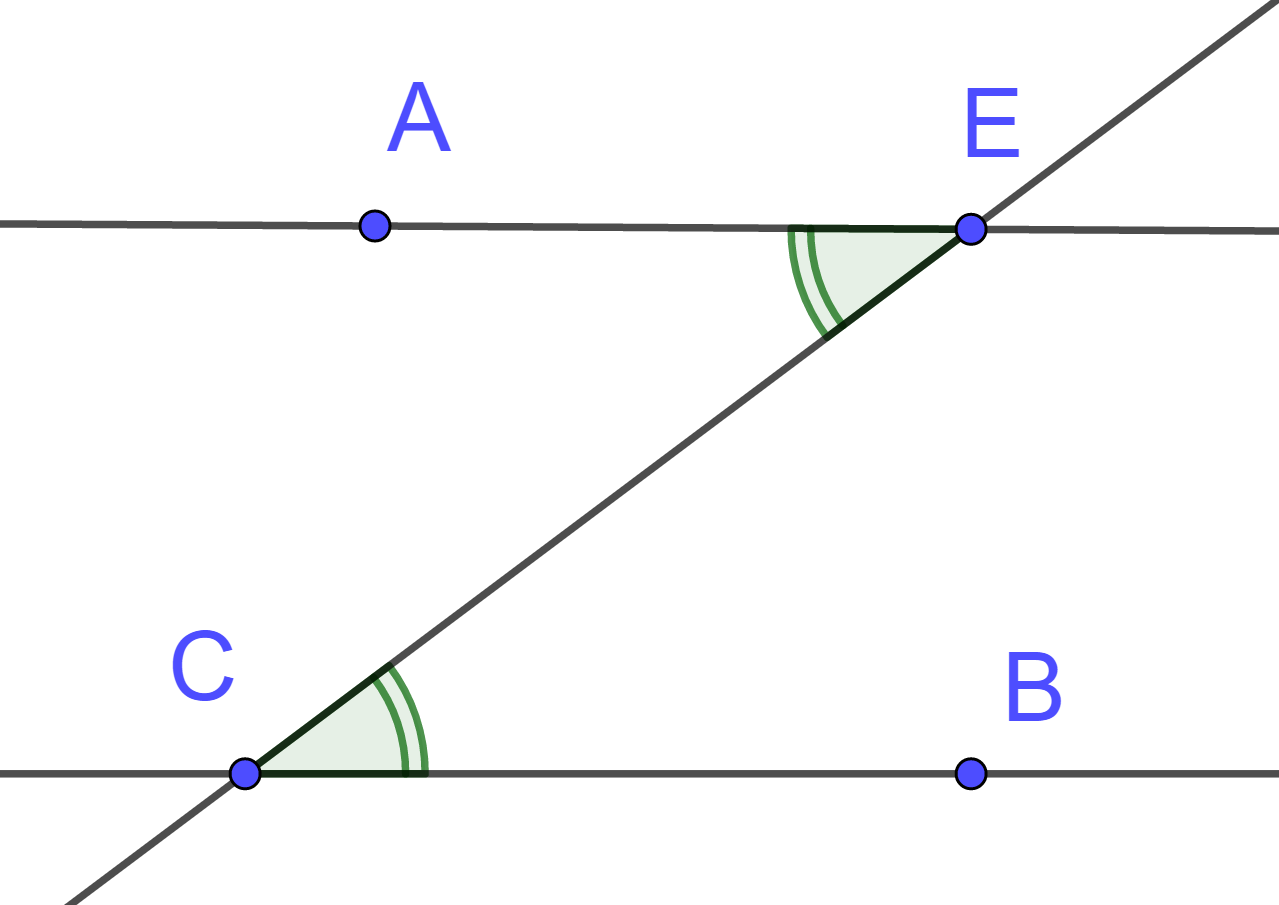
\includegraphics[scale=0.15]{alt_int3}
		\end{center}
	\end{multicols}
\end{myex}



\section{Angles correspondants}


\begin{mydef}
	
	
	Soit deux droites $(d_1)$ et $(d_2)$, une troisième droite $(s)$, les coupe en $A$ et $B$.
	Dans angles formés par ces 3 droites sont correspondants si et seulement si :
	
	\begin{multicols}{2}
		\begin{itemize}
			\item ils ont pour sommet $A$ et $B$;
			\item ils sont du même côté de la droite $(s)$;
			\item L'un est à l'intérieur des droites $(d_1)$ et $(d_2)$, l'autre à l'extérieur.
		\end{itemize}
		
		
		\begin{center}
			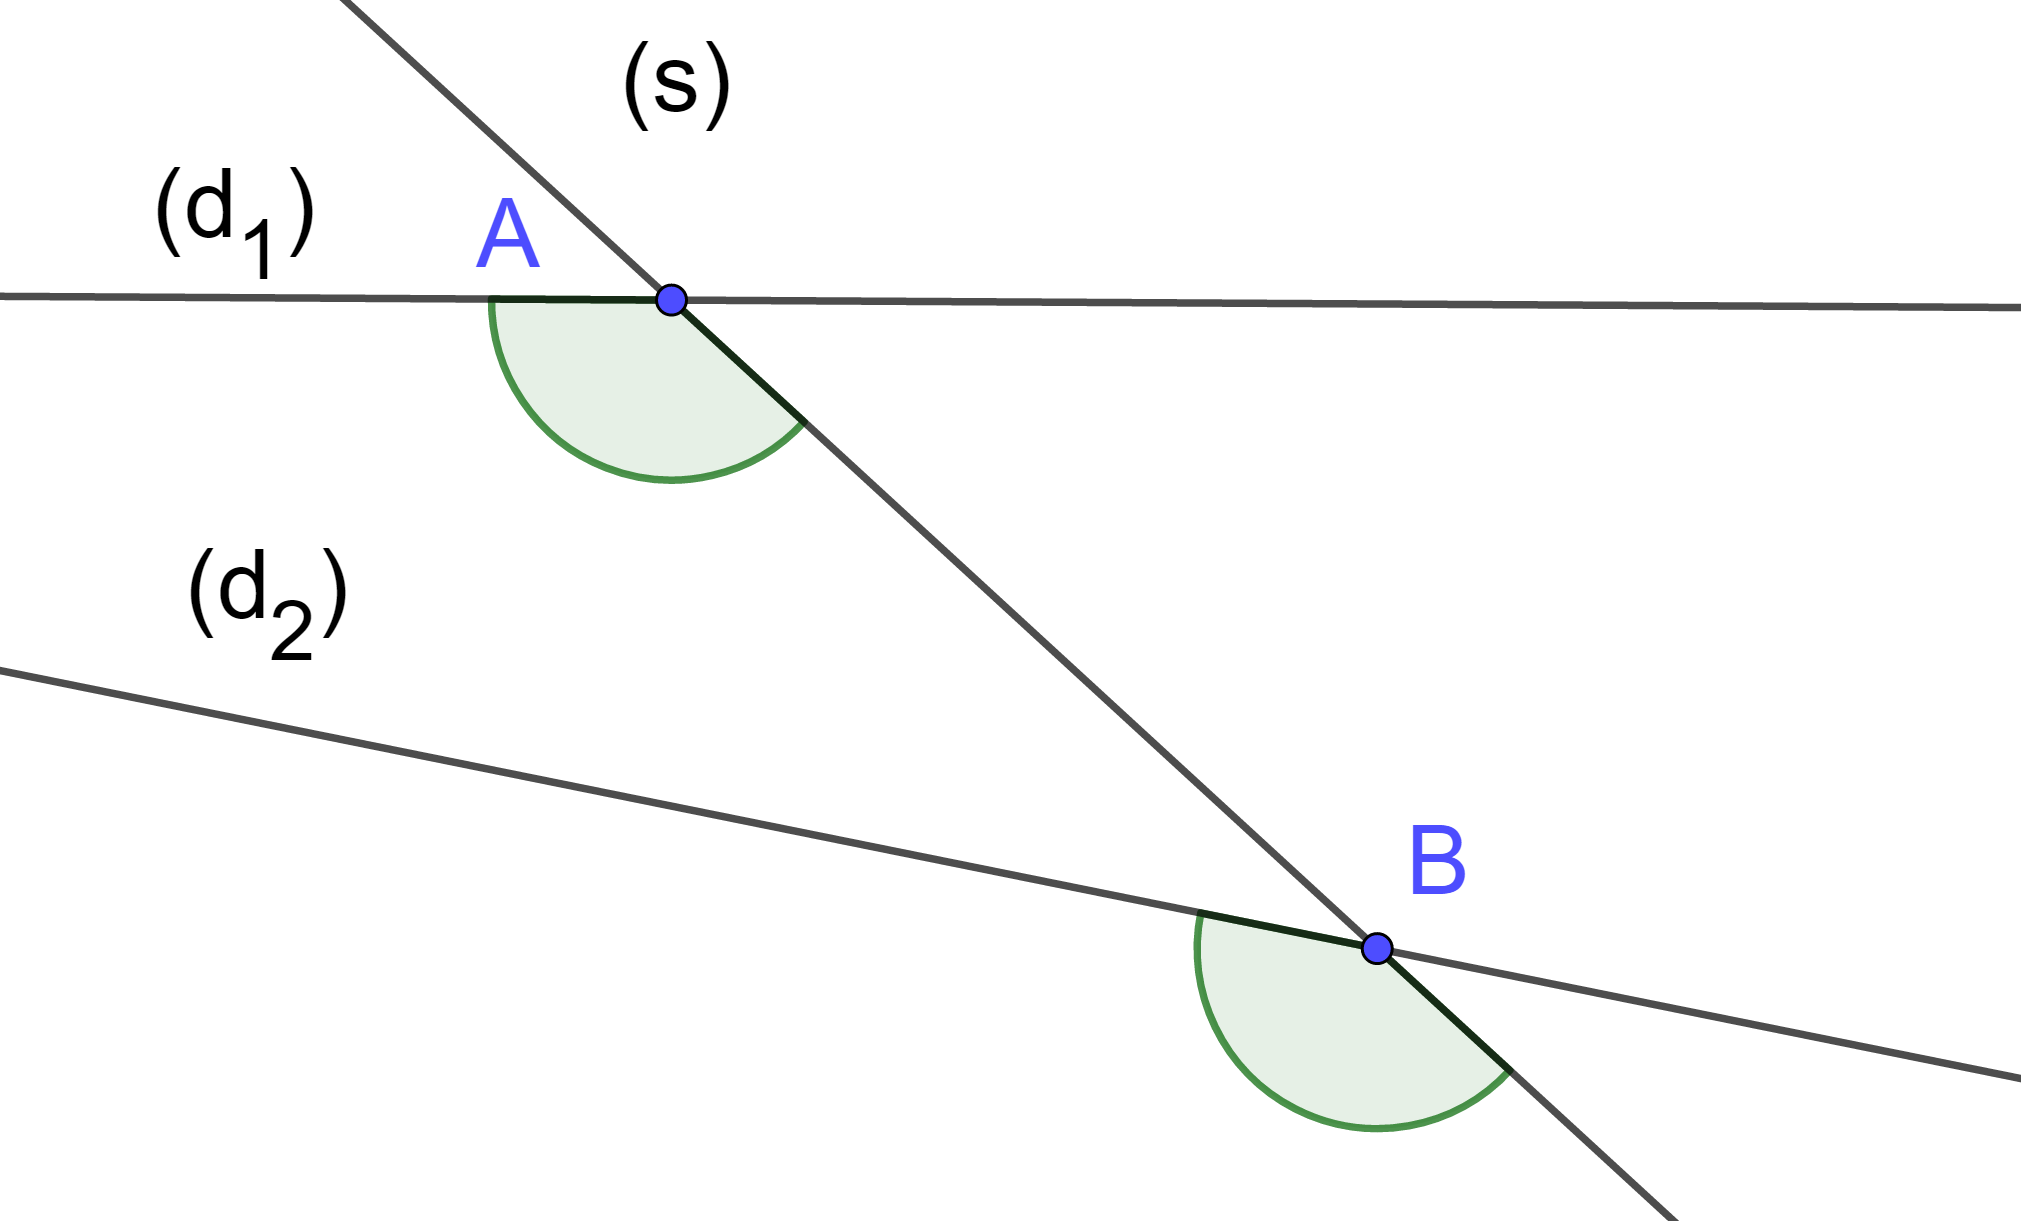
\includegraphics[scale=0.12]{corres}
		\end{center}
	\end{multicols}
	
\end{mydef}


\begin{myprop}
	Si deux droites coupées par une sécante sont \kw{parallèles}, alors les angles correspondants ont \kw{la même mesure}.
\end{myprop}

\begin{myex}
	
	
	\begin{multicols}{2}
		Les droites $(AF)$ et $(BC)$ sont parallèles et les angles $\widehat{DAF}$ et $\widehat{ABC}$ sont correspondants. \\
		
		Donc les angles $\widehat{DAF}$ et $\widehat{ABC}$ ont la même mesure.
		
		\begin{center}
			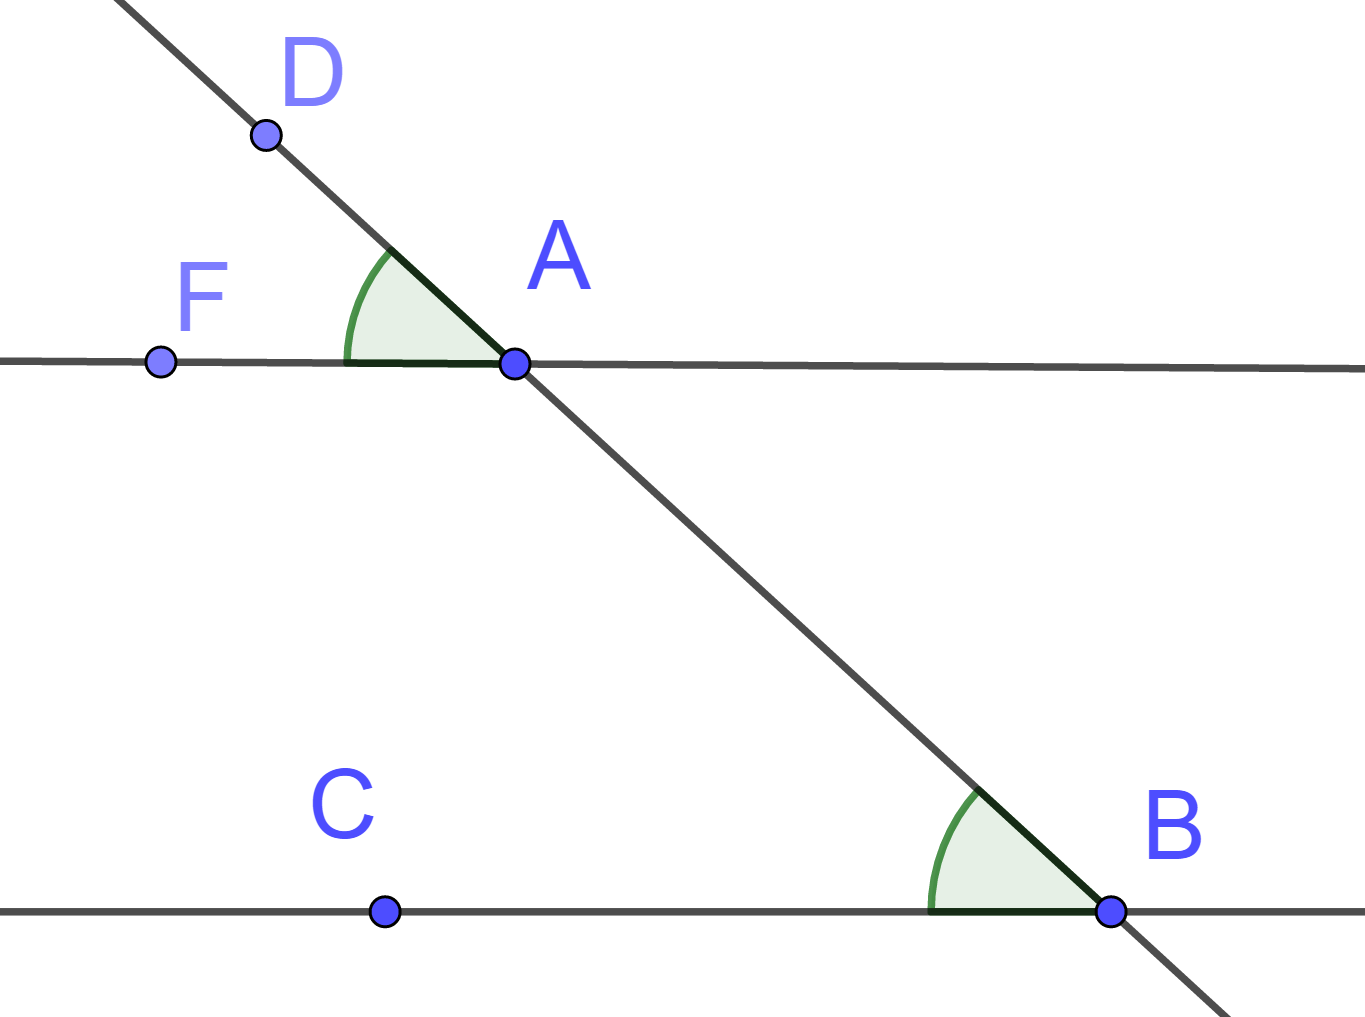
\includegraphics[scale=0.14]{corres2}
		\end{center}
	\end{multicols}
\end{myex}


\begin{myprop}
	Si deux angles correspondants ont \kw{la même mesure}, alors les droites coupées par la sécante sont \kw{parallèles}.
\end{myprop}

\begin{myex}
	\begin{multicols}{2}
		
		Les angles $\widehat{FAB}$ et $\widehat{GBD}$ sont correspondants et de même mesure. \\
		
		Donc les droites $(AF)$ et $(BC)$ sont parallèles.
		
		\begin{center}
			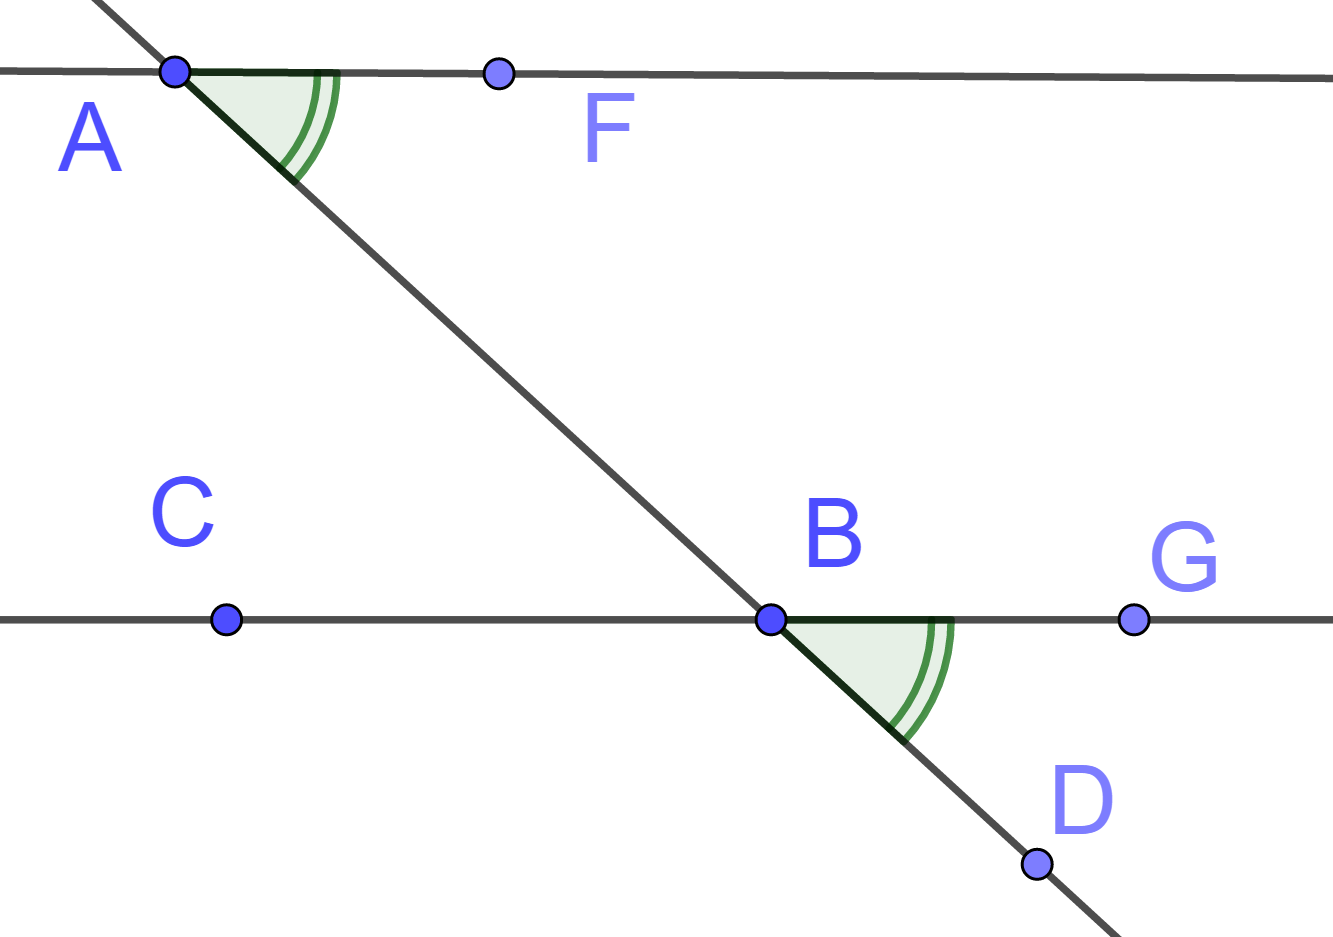
\includegraphics[scale=0.14]{corres3}
		\end{center}
	\end{multicols}
\end{myex}
\end{document}

